%%=============================================================================
%% Methodologie
%%=============================================================================

\chapter{\IfLanguageName{dutch}{Methodologie}{Methodology}}
\label{ch:methodologie}

\section{Uitleg termen}
In tabel 3.1 zijn termen terug te vinden die in dit hoofdstuk regelmatig zullen voorkomen.

\begin{table}[]
	\resizebox{\textwidth}{!}{%
		\begin{tabular}{|l|p{10cm}|}
			\hline 
			Queue & Een wachtrij waar berichten op geplaatst worden. Het bericht op de queue kan maar één keer gelezen worden. \\ \hline
			Consumption & De term om een bericht van de queue te lezen. \\ \hline
			Acknowledgement & Het verwijderen van een bericht op de queue. \\ \hline
			Overhead &  Als er teveel data aanwezig is op de queue dan spreekt men van overhead. Dit kan er voor zorgen dat de queue geen berichten meer ontvangt. \\ \hline
		\end{tabular}%
	}
	\caption{Termen die vaker voorkomen in dit hoofdstuk.}
\end{table}

\section{Communicatie methode}
\begin{figure}[h]
	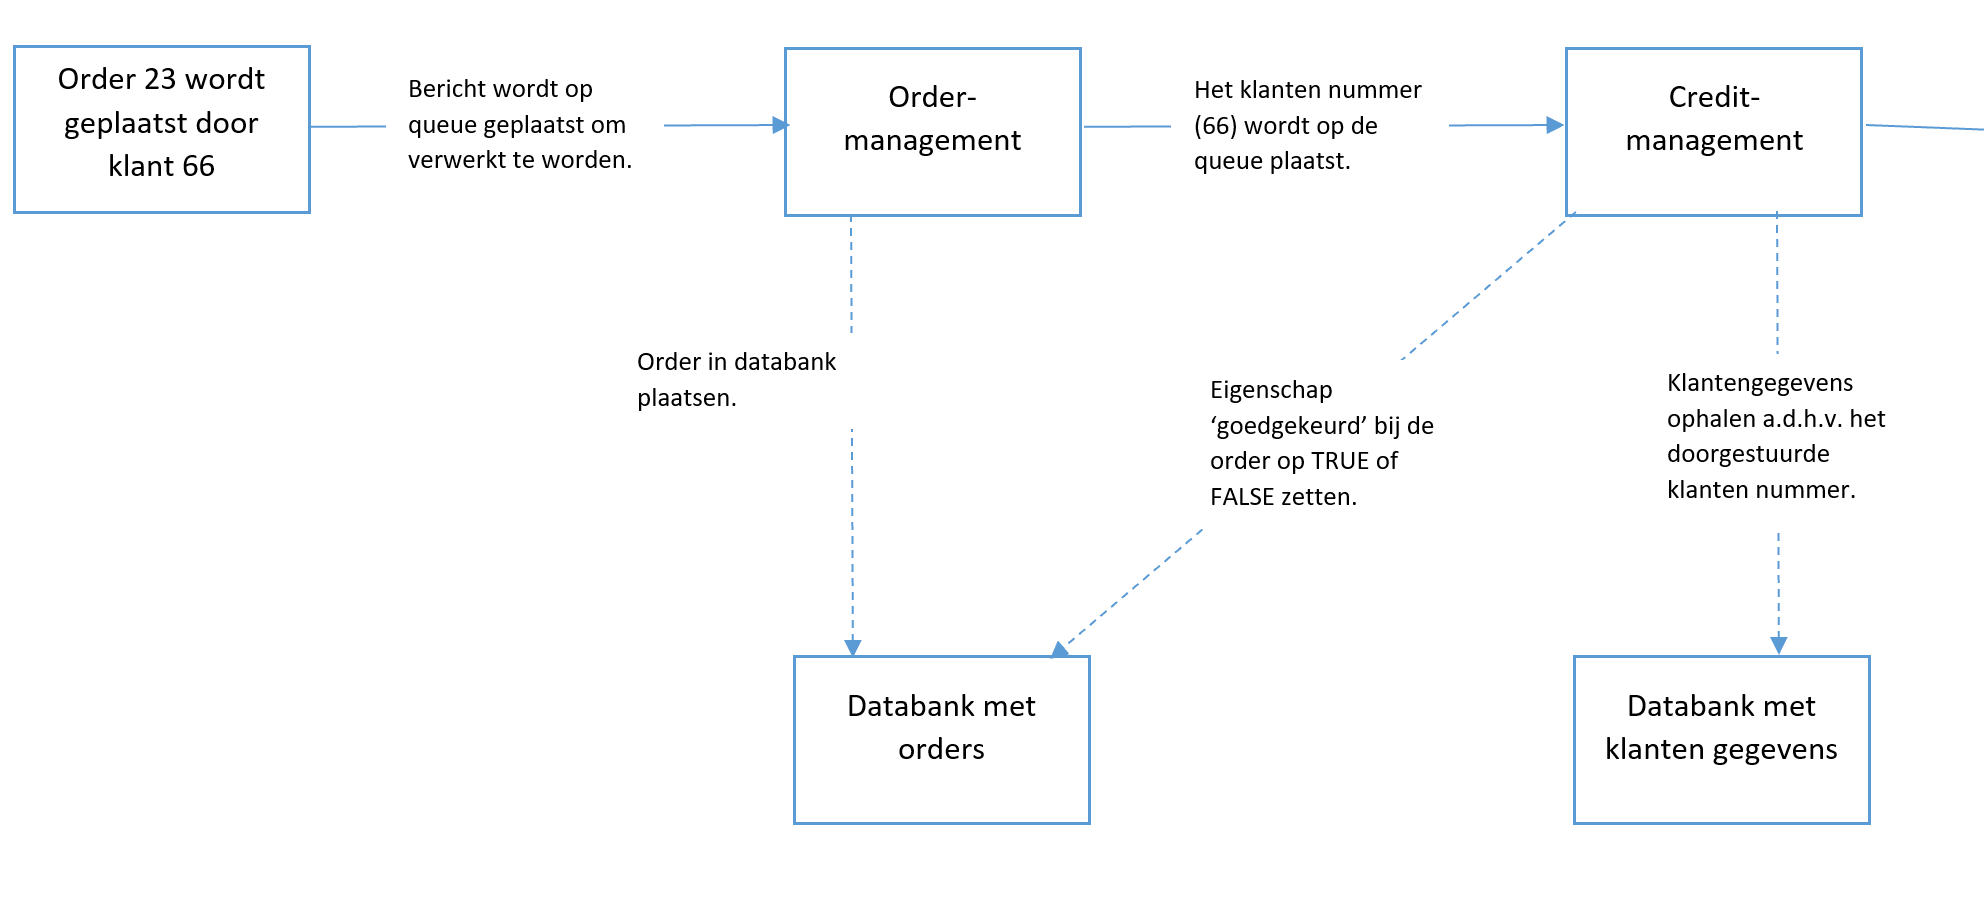
\includegraphics[width=10cm]{schemaEM.png}
	\caption{Hoe de messaging zou toegepast worden binnen het proces.}
	\centering
\end{figure}
Microservices moeten met elkaar kunnen communiceren. Bijvoorbeeld: Er wordt een order geplaatst door klant 66. Om na te gaan of die klant wel een order mag plaatsen, wordt de klant nummer doorgestuurd naar credit management. Om toch onafhankelijk van elkaar te blijven, gaan de microservices niet controleren of de data is aangekomen bij de andere microservices. De berichten worden op de queue van de microservice geplaatst. Dan is de microservice zelf verantwoordelijk voor het ophalen van hun data. Het ophalen van de data gebeurt via consumption en acknowledgement. Elke keer er een bericht geplaatst wordt op de queue, wordt de consumption en acknowledgement getriggerd om te gebeuren. Zo kunnen er meerdere credit controles gelijklopend gebeuren. 
Dus volgende queue's zouden moeten bestaan:
\begin{itemize}
	\item QorderMan is een queue voor order management: Het plaatsen van een order.
	\item QcreditMan is een queue voor credit management: Om te controleren of een klant wel een order mag plaatsen.
	\item QorderFul is een queue voor order fulfilment: Het ophalen van de order in het magazijn.
	\item QorderShip is een queue voor order shipment: Het plannen van de route en welke goederen op welke vrachtwagen moeten geladen worden.
	\item Qfact is een queue voor de facturatie.
	\item QaccountsRec is een queue voor accounts receivable: De betaling van de factuur nagaan en tijdig aanmaningen sturen. 
\end{itemize}

Niet alle data wordt volledig naar de queue gestuurd enkel de belangrijke data. Zoals bijvoorbeeld de klant die een order plaatste, die zijn klantnummer zal doorgestuurd worden naar credit management. Bij credit manangement wordt er dan aan de hand van het klantnummer de gegevens opgehaald en dan zo nagegaan of die klant wel een order mag plaatsen. Zo blijft de overhead op de queue minimaal. Om meer gegevens op te halen, moet de databank aangesproken worden. De gehele structuur van de databank wordt beschreven in het volgende gedeelte.

\section{De databank structuur}
Onderliggend is één grote databank waar alle masterdata in terug te vinden is. Hier is de enige plaats waar een single point-of-failure terug te vinden is. 
\begin{figure}[h]
	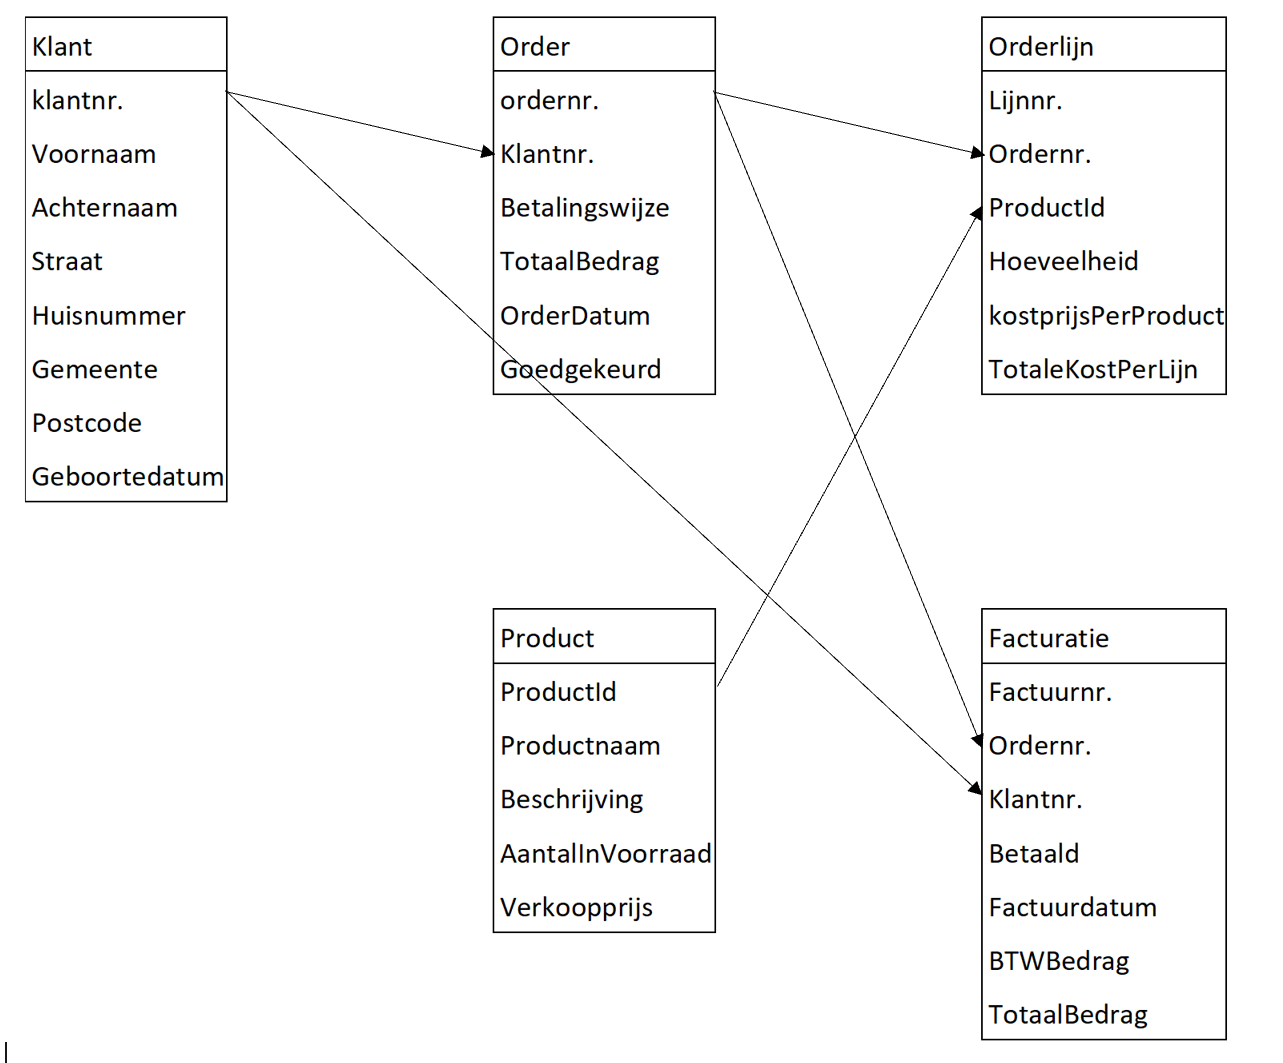
\includegraphics[width=10cm]{databank.png}
	\caption{De databank structuur.}
	\centering
\end{figure}

Een order weet wie zijn klant is. Dit is zodat het credit management de eigenschap bij de order kan veranderen van 'goedgekeurd' naar 'niet goedgekeurd'. Van elk order wordt ook een orderlijn bijgehouden. Zodat er geweten is wat er op de order staat. Op elk orderlijn staat er een product of service. Van het product moet er een beschrijving en verkoopprijs geweten zijn. Het aantal in voorraad is ook gekend omdat bij het order fullfilment moet de voorraad aangepast worden van het specifieke product. Een order en de klant zijn gekend op de facturatie. Zo kan er nagegaan worden of de factuur overeenkomt met wat er op het order staat. De klant zijn gegevens moeten gekend zijn om naar het juiste adres te factureren.


\section{De verschillende microservices}
Voor elk van volgende microservices gaan we volgende vragen beantwoorden:
\begin{itemize}
	\item Wat kunnen ze?
	\item Hoe ziet de databank eruit?
	\item Welk deeltje van de databank spreken ze aan?
	\item Waar kunnen ze gebruikt worden?
	\item Waarom werd hiervan een microservice gemaakt?
\end{itemize}

\subsection{Klantengegevens ophalen}
Deze microservice gaat ervoor zorgen dat de klantengegevens uit de databank worden gehaald. Het zal de databank aanspreken en vragen om de data van een specifieke klant. 
Hoe het schema van de databank er uit ziet, is terug te vinden in het vorige deel. 
Deze microservice wordt gebruikt in meerdere delen van het order-to-cash proces. Een van de voordelen van microservices is de schaalbaarheid. Omdat de requirement meermaals zal voorkomen in het proces, is het voordeliger om de microservice te dupliceren en te hergebruiken. 
Deze microservice komt voor in volgende onderdelen:
\begin{itemize}
	\item Order management
	\item Credit management
	\item Klant management
	\item Facturatie
	\item Accounts receivables
\end{itemize}

\subsection{Orders plaatsen, ophalen en verwijderen}
Een belangrijk onderdeel is het plaatsen, ophalen en verwijderen van orders. Deze microservice heeft verschillende verantwoordelijkheden en rechten op de databank. 
Deze microservice zal gebruikt worden in volgende onderdelen:
\begin{itemize}
	\item Order management
	\item Order fullfilment
	\item Facturatie
\end{itemize}

\subsection{Producten ophalen en het aantal in voorraad veranderen}
In het order-to-cash proces worden er geen producten toegevoegd aan de lijst dus moet dit niet in een microservice gestoken worden. Het aantal van de voorraad moet worden aangepast wanneer er een product uit de rekken wordt gehaald en bij een bestelling wordt geplaatst. Het ophalen van producten is vooral voor het werk achter de schermen. Het ophalen van een product omvat vooral de verkoopprijs ophalen om die dan te gebruiken in de orderlijn. 
Deze microservice zal gebruikt worden in volgende onderdelen:
\begin{itemize}
	\item Order management
	\item order fullfilment
\end{itemize}

\subsection{Facturatie maken en ophalen}
Het begin van het einde in een order-to-cash proces. Facturen maken en ophalen zijn van groot belang bij een order-to-cash proces. Het zorgt er voor dat mensen geld gaan betalen voor hun order. Een factuur moet overeenstemmen met wat geleverd is. Het is van groot belang dat achter kan gekeken worden of de factuur ook klopt met de order. Het maken van de factuur gebeurt ook aan de hand van het order. 
Deze microservice komt voor in het onderdeel facturatie.

\subsection{Shipment documentatie opstellen}
Het shipment document wordt gegenereerd afhankelijk van het order. Er wordt gekeken naar het ordernummer en dan wordt er gekeken naar het klantnummer. Hierna wordt dan de microservice om klantgegevens op te halen aangesproken om de gegevens van de specifieke klant op te halen. Dit wordt enkel gebruikt binnen het onderdeel verzending.

\subsection{Aanmaning opmaken en verwijderen}
Het opmaken en verwijderen van aanmaningen gebeurt enkel wanneer een wanbetaler is. Het proces zou niet vaak mogen voorkomen. 



\section{De complete architectuur opbouwen}
Stap per stap in het proces alles aanhalen
\begin{itemize}
	\item welke microservices aanspreken
	\item waarom?
\end{itemize}



